\documentclass[dvipsnames]{standalone}
\usepackage{tikz}

\begin{document}

    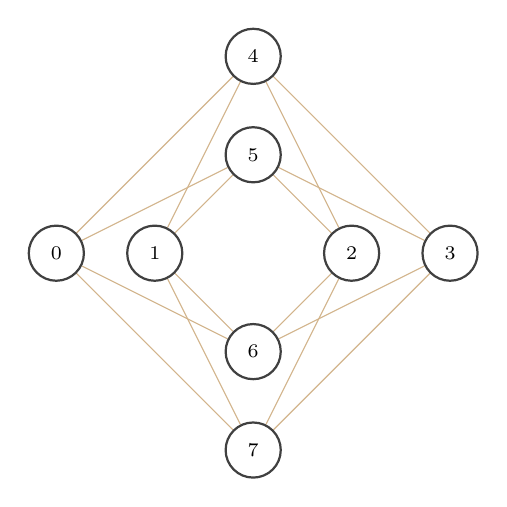
\begin{tikzpicture}[
        scale=0.25,
        coupler/.style={draw},
        qubit/.style={circle, thick, font={\scriptsize}, fill=White,draw=darkgray,minimum size=7mm, inner sep=0.5mm},
        hidden/.style={opacity=0.0},
        external/.style={color=RoyalBlue, thin},
        internal/.style={color=Tan, thin},
    ]

    \node[qubit, hidden] (0) at (0.0, -10.0) { 0 };
    \node[qubit, hidden] (4) at (10.0, 0.0) { 4 };
    \node[qubit, hidden] (5) at (10.0, -5.0) { 5 };
    \node[qubit, hidden] (6) at (10.0, -15.0) { 6 };
    \node[qubit, hidden] (7) at (10.0, -20.0) { 7 };
    \node[qubit, hidden] (1) at (5.0, -10.0) { 1 };
    \node[qubit, hidden] (2) at (15.0, -10.0) { 2 };
    \node[qubit, hidden] (3) at (20.0, -10.0) { 3 };
    \path[coupler, internal] (0) edge (4);
    \path[coupler, internal] (0) edge (5);
    \path[coupler, internal] (0) edge (6);
    \path[coupler, internal] (0) edge (7);
    \path[coupler, internal] (4) edge (1);
    \path[coupler, internal] (4) edge (2);
    \path[coupler, internal] (4) edge (3);
    \path[coupler, internal] (5) edge (1);
    \path[coupler, internal] (5) edge (2);
    \path[coupler, internal] (5) edge (3);
    \path[coupler, internal] (6) edge (1);
    \path[coupler, internal] (6) edge (2);
    \path[coupler, internal] (6) edge (3);
    \path[coupler, internal] (7) edge (1);
    \path[coupler, internal] (7) edge (2);
    \path[coupler, internal] (7) edge (3);
    \node[qubit] (0-front) at (0.0, -10.0) { 0 };
    \node[qubit] (4-front) at (10.0, 0.0) { 4 };
    \node[qubit] (5-front) at (10.0, -5.0) { 5 };
    \node[qubit] (6-front) at (10.0, -15.0) { 6 };
    \node[qubit] (7-front) at (10.0, -20.0) { 7 };
    \node[qubit] (1-front) at (5.0, -10.0) { 1 };
    \node[qubit] (2-front) at (15.0, -10.0) { 2 };
    \node[qubit] (3-front) at (20.0, -10.0) { 3 };
    \end{tikzpicture}

\end{document}